%%%%%%%%%%%%%%%%%%%%%%%%%%%%%%%%%%%%%%%%%%%%%%%%%%%%%%%%%%%%%%%%%%%%%%%%%%%%%%%%%%%%%%%%%%%%%%%%%%%%%%%%%%%%%%%%%%%%%%%%%%%%%%%%%%%%%%%%%%%%%%%%%%%%%%%%%%%
% This is just an example/guide for you to refer to when submitting manuscripts to Frontiers, it is not mandatory to use Frontiers .cls files nor frontiers.tex  %
% This will only generate the Manuscript, the final article will be typeset by Frontiers after acceptance.                                                 %
%                                                                                                                                                         %
% When submitting your files, remember to upload this *tex file, the pdf generated with it, the *bib file (if bibliography is not within the *tex) and all the figures.
%%%%%%%%%%%%%%%%%%%%%%%%%%%%%%%%%%%%%%%%%%%%%%%%%%%%%%%%%%%%%%%%%%%%%%%%%%%%%%%%%%%%%%%%%%%%%%%%%%%%%%%%%%%%%%%%%%%%%%%%%%%%%%%%%%%%%%%%%%%%%%%%%%%%%%%%%%%

%%% Version 3.1 Generated 2015/22/05 %%%
%%% You will need to have the following packages installed: datetime, fmtcount, etoolbox, fcprefix, which are normally inlcuded in WinEdt. %%%
%%% In http://www.ctan.org/ you can find the packages and how to install them, if necessary. %%%

\documentclass{frontiersSCNS} % for Science, Engineering and Humanities and Social Sciences articles
%\documentclass{frontiersHLTH} % for Health articles
%\documentclass{frontiersFPHY} % for Physics and Applied Mathematics and Statistics articles

%\setcitestyle{square}
\usepackage{url,hyperref,lineno,microtype}
\usepackage[onehalfspacing]{setspace}
\usepackage{subcaption}

\linenumbers


% Leave a blank line between paragraphs instead of using \\


\def\keyFont{\fontsize{8}{11}\helveticabold }
\def\firstAuthorLast{Moron {et~al.}} %use et al only if is more than 1 author
\def\Authors{Odin Moron\,$^{1,*}$, x\,$^{{2}}$, y\,$^{{3,*}}$}
% Affiliations should be keyed to the author's name with superscript numbers and be listed as follows: Laboratory, Institute, Department, Organization, City, State abbreviation (USA, Canada, Australia), and Country (without detailed address information such as city zip codes or street names).
% If one of the authors has a change of address, list the new address below the correspondence details using a superscript symbol and use the same symbol to indicate the author in the author list.
\def\Address{$^{1}$National Plant Phenomics Centre, IBERS, Aberyswyth University, Gogerddan, Aberystwyth, SY23 3EB, UK\\
$^{3}$ x\\ $^{2}$ y}
% The Corresponding Author should be marked with an asterisk
% Provide the exact contact address (this time including street name and city zip code) and email of the corresponding author
\def\corrAuthor{x}
\def\corrAddress{x}
\def\corrEmail{x}

\newcommand{\todo}[1]{
  \rule{0pt}{0pt}\marginpar{{\color{blue}\rule{1ex}{1ex}}}
  {[\textbf{\color{blue}todo:} #1]}}


\begin{document}
\onecolumn
\firstpage{1}

\title[Effects of Segmentation Quality on Shape Descriptors]{Effects of Segmentation Quality on Shape Descriptors} 

\author[\firstAuthorLast ]{\Authors} %This field will be automatically populated
\address{} %This field will be automatically populated
\correspondance{} %This field will be automatically populated

\extraAuth{}% If there are more than 1 corresponding author, comment this line and uncomment the next one.
%\extraAuth{corresponding Author2 \\ Laboratory X2, Institute X2, Department X2, Organization X2, Street X2, City X2 , State XX2 (only USA, Canada and Australia), Zip Code2, X2 Country X2, email2@uni2.edu}


\maketitle


\begin{abstract}

\tiny
 \keyFont{ \section{Keywords:} computer vision; arabidopsis; machine learning; phenomics } %All article types: you may provide up to 8 keywords; at least 5 are mandatory.
\end{abstract}

\section{Introduction}

Image segmentation is the process of identifying and delineating objects in images. Segmentation techniques are used to separate the region of interest (ROI) from the remainder of the image. Image segmentation is critical as it is the major step demarcating between ROI and the background \cite{Rathnayaka2011226} and thus, has a major effect over the calculation of shape descriptors which are produced to describe a given shape. Due to the advent of computer technology image-processing techniques have become increasingly important in a wide variety of applications. \todo{explain why is important in phenomics}

Image segmentation may be thought of as consisting of two related processes—recognition and delineation. Recognition is the high-level process of determining roughly the whereabouts of an object of interest in the image \cite{Udupa200675}. Delineation is the low-level process of determining the precise spatial extent and point-by-point composition (material membership percentage) of the object in the image. Humans are more qualitative and less quantitative, whereas, computerised algorithms are more quantitative and less qualitative. Incorporation of high-level expert human knowledge algorithmically into the computer has remained a challenge. Most of the drawbacks of current segmentation methods may thus be attributed to the latter weakness of computers in the recognition process. We envisage, therefore, that the assistance of humans, knowledgeable in the application domain, will remain essential in any practical image segmentation method. The challenge and goal for image scientists are to develop methods that minimize the degree of this required help as much as possible.

While algorithms for image segmentation have been in development for several decades \cite{ZAITOUN2015797}, the development of systematic evaluation frameworks for these algorithms has been lagging, particularly in plant phenotyping. In this paper, two segmentation methods are compared against manually segmented images, to assess the role of segmentation quality in the measurement of the shape descriptor. A segmentation workflow in Lemnagrid \cite{ISI:000245413900027} has been created such that it is more prone to miss plant pixels from foreground than accept alien pixels into it. A Matlab \cite{MATLAB:2010} script has been written in a way that it is accurate classifying plants but accepts pieces of the background as plant more often (higher rate of false negatives); In addition, it also miss larger leaves extremes that are close to the pot border.

Each segmentation routine has first been evaluated in terms of classification quality, and later their shape descriptor accuracy. This strategy allows to conclude that including segmentation artefacts reduce precision of shape descriptors more than missing plants, at least when segmentation errors are not very big. It is possible to suggest that experimental systems have to be set up to ease image segmentation at least to eliminate as much as possible misclassification of background pixels.

%\begin{methods}
\section{Material \& Methods}

\todo{}
Arabidopsis thaliana top-view pictures have been segmented either as rosettes or background \ref{fig1:segmentation}. Briefly, each pixel should belong to one of two classes e.g. foreground (1) and background (0). Strictly speaking, foreground pixels represent the plant and background pixels represent all other elements in the image, e.g. stones, pot and soil. Due to similarity in colours between plant and other image elements, plant pixels may be not classified correctly. Common culprits of misclassification are yellow or grey regions on leaves, pieces of soil or stones on top of plant leaves and thin petioles. Likewise, background pixels may be misclassified as foreground. Examples misclassified background objects are pixels corresponding to moss or algae growing on the soil surface and whose colour is similar to the target foreground (the plant). Other examples are stones and plastic pieces and pot edges \ref{fig1:segmentation}.

\subsection{Phenotyping}


\subsection{Shape descriptors}

In general, descriptors are some set of numbers that are produced to describe a given shape. The shape may not be
entirely reconstructable from the descriptors, but the descriptors for different shapes should be different enough that
the shapes can be discriminated.
What qualifies as a good descriptor? In general, the better the descriptor is, the greater the difference in the descriptors
of significantly different shapes and the lesser the difference for similar shapes. What then qualifies similarity
of shape? Well, nobody’s really been able to answer that one yet. If we could quantify similarity of shape, we’d have
the perfect descriptor. Indeed, that’s what descriptors are: attempts to quantify shape in ways that agree with human
intuition (or task-specific requirements). Regions can either describe boundary-based properties of an object or they can describe region-based properties. 
 \cite{}
\todo{Can you out examples of shape descriptors?}

\subsection{Segmentation Pipeline}

Two automatic segmentation pipelines has been tested. Lemnatec (LT) workflow was performed using LemnaGrid Software \cite{ISI:000245413900027}. It consists on image analysis in three separate sub-routines. One extracts metallic tags on pots borders by eliminating very bright pixels. Another looks for plant pixels based on colour transformations and subsequent global thresholding. The third routine removes other bright elements such as plastic pots and stones.
Matlab (MA) pipeline consist in a script using Matlab’s Image Processing toolbox \cite{MATLAB:2010}. It searches in parallel for green pixels, those with green intensity over 60 units (up to a maximum of 255), and for pixels whose green intensity is higher than red intensity. The aim was to keep leaves at the time that remove bright objects, but keeping those that maintain their green intensity. Thus, green and yellow leaves are classified as leaves, but yellow-reddish stones are removed. However, to avoid many plastic pot pixels included as foreground, pots borders were trimmed through a mathematical morphology operation called erosion. Border erosion impose to miss some leaves extremes counting as False Negatives, and it is still not able to get rid of all the pots pixels. Therefore, in spite of Matlab routine is far from optimal, it allows to study the effects of including segmentation artefacts of different size into Shape descriptors calculations.
Same  images has been segmented automatically with both methods. In addition, they were manually segmented using GIMP \cite{} to stablish a 'ground-truth' dataset (GT). Manually segmented images constitute a ground truth to compare both workflows against it.


\subsection{Segmentation evaluation}
Two ways of evaluating segmentation are studied in this section. First, segmentation quality is analysed by comparing by pixels each automatically segmented images with their ground truth. Second, Shape Descriptors errors are analysed as deviations from ground truth values.
For segmentation quality, an exploration using the number of false positives and false negatives is provided. Generally, comparing automatically segmented images, either Lemnatec or Matlab pipeline, against ground truth corresponding image, requires calculation the so called confusion matrix. A confusion matrix, see \cite{Fawcett:2006:IRA:1159473.1159475} for a review, summarize the number of true positives and negatives and the number of false positives and negatives are obtained. This matrix allows to calculate for a given method several metrics that aid into quantify segmentation errors. This metrics are summarize in box 1 for readers convenience. 
Typically, confusion matrix derived parameters are plotted and analysed to compare between classification algorithms and the values of their parameters to assess which method or set of parameters perform better. However, in here, confusion matrix is used in a heterodox manner to improve the visualization of segmentation mistakes. Figure 3 shows a scatter plot where False Negative Rate is plotted against the False Discovery Rate (see below). Each point corresponds to an image, instead of summarizing a method. Both methods are represented in red and blue colours for comparison purposes.
In the image segmentation context, Negatives are considered as pixels belonging to the background and Positives as foreground. The False Negative Rate (FNR hereafter) is defined as the number of False Negatives divided over the overall number of Positives (Box 1). Thus, FNR indicates the percentage of plant pixels that has been classified as background out of the real number of plant pixels. Therefore, it is the rate of plant pixels lost over the total number of plant pixels. On the other hand, the False Discovery Rate (FDR hereafter), as False Positive over the overall number of Positives (see Box 1). FDR indicates the percentage of background pixels classified as foreground over the total of real foreground pixels. Therefore, it represent the percentage of artefact pixels present in the segmented image over the number of plant pixels, classified as plants or not.
Deviation of Shape descriptor values from ground truth ones helps testing the effects of segmentation errors on the descriptors. The effects are quantified accounting the relationship of errors with the confusion matrix metrics. For every shape descriptor, the value of the parameter is plotted, for both methods, against the ground standard value. A paired t-test (Welsh test) is used then to evaluate if differences are significant (tables 1, 2 and 3). Scatter plots of descriptor differences between automatically and manually segmented images, against False Discovery Rate and False Negative Rate are provided. For scatter plots of FDR against error, the correlation for positive valued errors and FDR is calculated and plotted. For FNR against error scatter plots, correlation for negative valued errors and FNR is then provided.



%\begin{table}[!t]
%\textbf{\refstepcounter{table}\label{Tab:02} Table \arabic{table}.}{ Infection type score table}\\
%\processtable{}
%{\begin{tabular}{l|l}
%\hline
%	score & description \\\midrule
%	0 & No visible symptoms \\
%	1  & Small, sporulating uredia surrounded by necrotic tissue \\
%	2 & Small, sporulating uredia surrounded by necrotic tissue \\
%	3 & Medium sized, sporulating uredia surrounded only by chlorotic tissue \\
%	4 & Large, sporulating uredia surrounded by green tissue \\ \hline
%\end{tabular}}{}
%\end{table}


\subsection{Statistics }
\todo{Can you comment on stats here e.g. software, methods, data normalisation, etc}

\section{Results}

An overview on the results indicated that Lemnatec pipeline performed well to remove artefacts \todo{(e.g. ????)}, but seems to fail to capture all leaves and petioles. The Matlab pipeline could remove soil and stones, but had problems segmenting metallic tags, pot's edges and leaves close to the pot's edge. Henceforth, they are two examples of segmentation, but the Matlab script shows the effect of those artefacts on the real values.


\subsection{Image Segmentation Quality}
Visual exploratory analysis of \ref{fig1:segmentation} shows the False Negative Rate against the False Discovery Rate \todo{Can you show evidence to support this statement?}. Each point correspond to a rosette image. It shows that Lemnatec pipeline has a low False Discovery Rate, indicating that few artefacts are included in the segmentation. However, the range on the False Negative Rate indicate that some images may have lost up to 60\% of the plant. The Matlab pipeline, seems to perform better on the False Negative Rate, since most of the images keep the pixel lost under the 20\%. However, the False Discovery Rate shows that the pipeline let some artefacts to be included, but those does not exceed the 2\%. 
Figure 3: Scatter plot of False Negative Rate against False Discovery rate for segmentation routines called “Lemnatec” and “Matlab”. Note: Each dot corresponds to an image. All images were segmented with “Lemnatec” and “Matlab” routines and matched against a manual segmentation called ground truth

\subsection{Effects on Shape descriptors}
As seen in the Material and Methods, Shape descriptors can deviate from their values. When objects other than plants are included, the effect on shape descriptors may greatly depends on the distance between plant outline and the object. The distance from artefacts to plant pixels is not explored here.
Projected Rosette Area
Regarding the Projected Rosette Area automatically segmented images tend to return lower values than the manual ground truth due to losses in plant pixels. For both methods differences against ground truth are significant (see table 1 and 2), as well as between methods. 
For Matlab routines, segmented rosettes with larger Area than growth truth, due to artefacts, are slightly correlated with FDR (cor=0.3) and those with smaller Area values are correlated with the FNR (cor=-0.6). For Lemnatec routine, almost no segmented plant showed bigger Area than ground truth. This might be due to no inclusion of any artefact or because of the compensation between pixels included and missed. Yet, FDR does not correlate with any departure of PRA (cor = -0.0011), but FNR strongly does (cor = -0.76).
Convex Hull Area
Convex Hull Area values calculated from Lemnatec pipeline are closer to the ground truth than those calculated from Matlab, although their differences with the ground truth and between methods are significant.
 Some images segmented with Matlab routine have bigger Convex Hull than expected from ground truth, probably due to the inclusion of elements far from their leaves. These plants have ground truth values of convex hull between 50•104 and 10•105 pixels. For bigger plants, the convex hull calculated with Matlab routine are smaller, like rising to a plateau. This effect is due to Matlab routine accepts quite often pixels from pots border, which have a constant size in this image set.
Convex Hull Area errors, for Matlab pipeline, is slightly correlated with FDR (cor =0.38) for those images showing larger values than the ground truth. The FDR is not correlated with negative values of Convex Hull Area errors (Cor=-0.2). For Lemnatec routine, almost any image shows bigger Convex Hull Areas than ground truth, so no correlation make sense. Yet, correlation between Convex Hull Area and FDR for negative errors are correlated (Cor= -0.74).
\subsection{Compactness}
Compactness is biased by artefacts altering Convex Hull Area in both pipelines. Figure 4 seems to indicate that Matlab perform worse than Lemnatec for Compacness, but paired t-test does no confirm this (p-value for the differences between two methods =. 0.19 >0.05, see table 3), however, both methods are significantly different than ground truth. Matlab segmented images show more Compactness values smaller than the ground truth than bigger. Positive errors are less disperse than negative ones, and the correlation between positive values and FDR is only 0.12, and the correlation between negative values and FNR is -0.064. For lemnatec segmented images, almost no compactness values where bigger than ground truth, being the correlation value with FDR (Cor = -0.38) meaningless. On the other hand, Compacness values smaller than ground truth highly correlated with FNR (Cor = -0.96) indicating that the more missing pixels the smaller the Compactness.
\subsection{Perimeter}
Perimeter errors seems to be split in two sub-categories. Some images show errors relatively close to the ground truth, but many other has Perimeter reduced to very low values. Significant differences are found for every method against ground truth and among both methods. However, Lemnatec pipeline show a more continuous distribution of errors than Matlab routine. Perimeter values larger for automatically segmented images than for ground truth are slightly correlated with FDR for those analysed with Matlab (Cor = -0.47) but not for Lemnatec (Cor = -0.15). FNR does not correlate for both segmentation methods with their negative errors in Perimeter (Cor ~ -0.1 for both routines) due to the high dispersion in both axis.
\subsection{Roundness}
Roundness convey the behaviour of perimeter, used in its calculation. Many rosettes fall to a zero-valued roundness for both algorithms. Thus, both algorithms results are significantly different from ground truth, and among them. The FDR moderately correlates with Roundness positive errors for Matlab segmented images (Cor = -0.52) but not for Lemnatec ones (Cor = -0.19). FNR does not show correlation for both methods and negative errors(Matlab Cor = -0.3 and Lemnatec Cor = -0.02) . However, FNR seems to have positive correlation with positive values, which no explanation is available.

\subsection{Eccentricity, Rotational Moments and Principal Axis Ratio}
A different behaviour is observed in Eccentricity, Rotational moments and Principal Axis Ratio. They are three measurements about rosette departure from a circle and their values are difficult to interpret. Rotational moments values are close to the ground truth and no differences are observed between methods (t-test p-value = 0.57). Although Lemnatec error is significant (p-val=0.04) but Matlab does not (p-val=0.99). For Matlab segmented images, FDR correlates with positive values (Cor = 0.068), indicating that artefacts are modifying this value. Lemnatec segmented images contained very few artefact so that FDR does not correlate with positive errors(Cor=-0.21). FNR does not show correlation for both pipelines (Matlab Cor = -0.18), especially for Lemnatec one (Cor = -0.32), that almost does not depart from ground truth values.
\subsection{Eccentricity}
 Eccentricity is affected by segmentation errors significantly in both methods, but hypothesis testing does not confirm differences between methods (p-val=0.14), although Matlab produced more disperse results. Neither FDR nor FNR are correlated with errors in any of both pipelines.
Principal Axis Ratio
In the case of Principal Axis Ratio, values are dispersed for Matlab and Lemnatec, and the difference between methods is very close to be significant(t-test p-value = 0.054). Matlab values dispersion is larger at negative and positive errors than Lemnatec values. Both pipelines positive errors show a very small correlation with FDR (Matlab Cor = 0.044 and Lemna Cor = 0.0074). For negative errors, Matlab is barely correlated (Cor = -0.13) but Lemnatec is slightly correlated (Cor = -0.5).
\subsection{Maximum Diameter}
Maximum Diameter shows a different pattern for Lemnatec and Matlab pipelines. Lemnatec fits better to ground truth than Matlab does. At 400 pixels, there is a plateau corresponding to pot size in Matlab segmented images. Both methods show significant differences among them and individually against the ground truth. In Matlab, positive errors, those whose maximum diameters are bigger than the ground truth, slightly correlates with FDR (Cor = 0.39) against expected. The correlation is almost similar than that between FDR and positive errors in Maximum Diameter for Lemnatec segmented images, but due to the small number of points, correlation is meaningless. For negative errors, matlab segmented images does not show correlation with FNR (Cor = -0.15) but it does for Lemnatec segmented images (Cor = -0.74).


\section{Discussion}

\todo{from intro}
Segmentation quality affects shape descriptors values of rosette in different manners. False negatives reduce the projected rosette area, but may or may not affect other parameters. For example, missing sparse pixels on leaves blades and perimeter may not affect the calculation of Convex Hull, Compactness, etc. But if a whole leave disappear, e.g because of grey colour, that may affect all the shape measurements, since spatial pixel distribution is modified. On the other hand, false positive may have strong effect on determining Convex Hull and other parameters. A single pixel, if far from the plant limits, will increase the extent of the Hull and will influence Compactness, but may not have strong effects on Roundness or Eccentricity. A bigger object misclassified as plant, like stones or pot borders, will have stronger effect on perimeter, roundness or eccentricity.
\todo{from intro}

In this chapter, the relevance of segmentation to calculate shape descriptors has been explored. Two methods of segmentation, named Lemnatec and Maltlab, have been used to explore the effect of artefacts and absence of plant material in the segmented images. The Lemnatec pipeline used was elaborated focusing in the elimination of artefacts, with the counterpart of leaving out some plant material. Matlab pipeline was elaborated to keep most of plants, with the common miss of small petioles, but accepts alien objects as plant often. For plants spanning further than pots border, leaves extreme were also missed.
The effect of missing or adding some pixels does affect Area. It can be assumed that small size artefacts are dissolved when the number of plant pixels are big enough. However, missing plants pixels is important as observed in the correlation with false negative rate.
Shape descriptors require to calculate several other geometrical quantities as perimeter or convex hull. The lack of leaves reduce the perimeter and the artefacts enlarge the Convex hull. This image processing-driven bias is conveyed to the shape descriptors calculated from them, like Compactness and Roundness.
Convex Hull Area is positively biased when artefacts are away from the plant, but not very dependent of the size of the artefact. This is represented with a low correlation between positive errors and the false discovery rate. On the other hand, missing plant pixels only have effect on convex hull when they correspond to whole parts like a full leave. This assertion can be extrapolated from the comparison among Lemnatec and Matlab pipelines against False Negative Rate. Since Lemnatec routine miss small pieces of leaves and petioles, its errors are closer to zero and the variation is very much related with the false negative rate. For the Matlab routine, the dispersion is larger and those with bigger errors are not those that have larger number of false negatives. A similar patter occurs in Compactness due to higher variation in errors for the Convex Hull than for Area. A look to the error plots in Compactness is visible that for a initially accurate pipepline as Lemnatec segmentation routine, Compactness can vary up to 20\%, but for a not that accurate one, Matlab routine, it rise to 50\%. This fact induce a thought that Compactness have to be studied with care due to a possible low signal to noise ratio.
Perimeter and Roundness.
Other Shape descriptors are not very affected by segmentation errors in the set of images under study. They are related with the departure of a circle and are calculated from the moments of all pixels and centroid. Examples of these descriptors are the Eccentricity, Principal Axis Ratio and Rotational Moment.
Finally, descriptors like Maximum Diameter, that provide a measure of the leaves span are can be biased only for plants of certain size but not for other.
The method proposed here to study the quality of the segmentation does not allow to know neither artefacts number, size and distance, nor if not segmented plant pixels belong to some region or are sparse. This could be relevant to study in order to know the particular kind of mistakes to be avoided. There are tools proposed to study segmentation border positioning error from ground truth, as those described by Sonka et al. quantifying the Hausdorff distance between borders in segmented images and ground truth.
The experience on automatic image segmentation dictates that most of the errors are due to similarities in colour or texture between classes, partially due to illumination. Improvements can be achieved by improving technicalities on computer vision algorithms and photography. However, experimental set up can adapt to post-processing in order to facilitate it. Examples could be using blue sand or blue mats on top of the soil, adjusting and homogenizing lights and avoid high reflective materials. In the context of Infrared and Fluorescence imaging some corrections has been tested by \cite{fpls.2014.00770}.


\section*{Disclosure/Conflict-of-Interest Statement}


The authors declare that the research was conducted in the absence of any commercial or financial relationships that could be construed as a potential conflict of interest.

\section*{Author Contributions}



\section*{Acknowledgments}
 We are grateful to the team of “National Plant Phenomics Centre” for carrying out the experiments and to the 
\textit{Funding\textcolon} for finantially suportting the project.



\bibliographystyle{frontiersinSCNS_ENG_HUMS} % for Science, Engineering and Humanities and Social Sciences articles, for Humanities and Social Sciences articles please include page numbers in the in-text citations
%\bibliographystyle{frontiersinHLTH&FPHY} % for Health and Physics articles
\bibliography{bioinfo}

%%% Upload the *bib file along with the *tex file and PDF on submission if the bibliography is not in the main *tex file

\section*{Figures}

%%% Use this if adding the figures directly in the mansucript, if so, please remember to also upload the files when submitting your article
%%% There is no need for adding the file termination, as long as you indicate where the file is saved. In the examples below the files (logo1.jpg and logo2.eps) are in the Frontiers LaTeX folder
%%% If using *.tif files convert them to .jpg or .png

%\begin{figure}
%    \begin{center}
%    \begin{subfigure}[b]{0.5\textwidth}
%        \includegraphics[width=\textwidth]{smarthouse.jpg}
%        \caption{Plant watering at gravimetrix level}
%       % \label{fig:tiger}
%    \end{subfigure}
%    ~ %add desired spacing between images, e. g. ~, \quad, \qquad, \hfill etc. 
%    %(or a blank line to force the subfigure onto a new line)
%    \begin{subfigure}[b]{0.5\textwidth}
%        \includegraphics[width=\textwidth]{scoring.jpg}
%        \caption{Plant scoring for developmental stages}
%        %\label{fig:mouse}
%    \end{subfigure}
%\end{center}
%    \caption{Contrast beween two lines whose disease score was four. Red vertical line indicates the date senescence on Flag leaf was first seen}\label{fig3}
%%\textbf{\refstepcounter{figure}\label{fig:03} Figure \arabic{figure}.}{Contrast beween two lines whose disease score was four. Red vertical line indicates the date senescence on Flag leaf was first seen}
%\end{figure}
%
%
\begin{figure}[h!]
\begin{center}
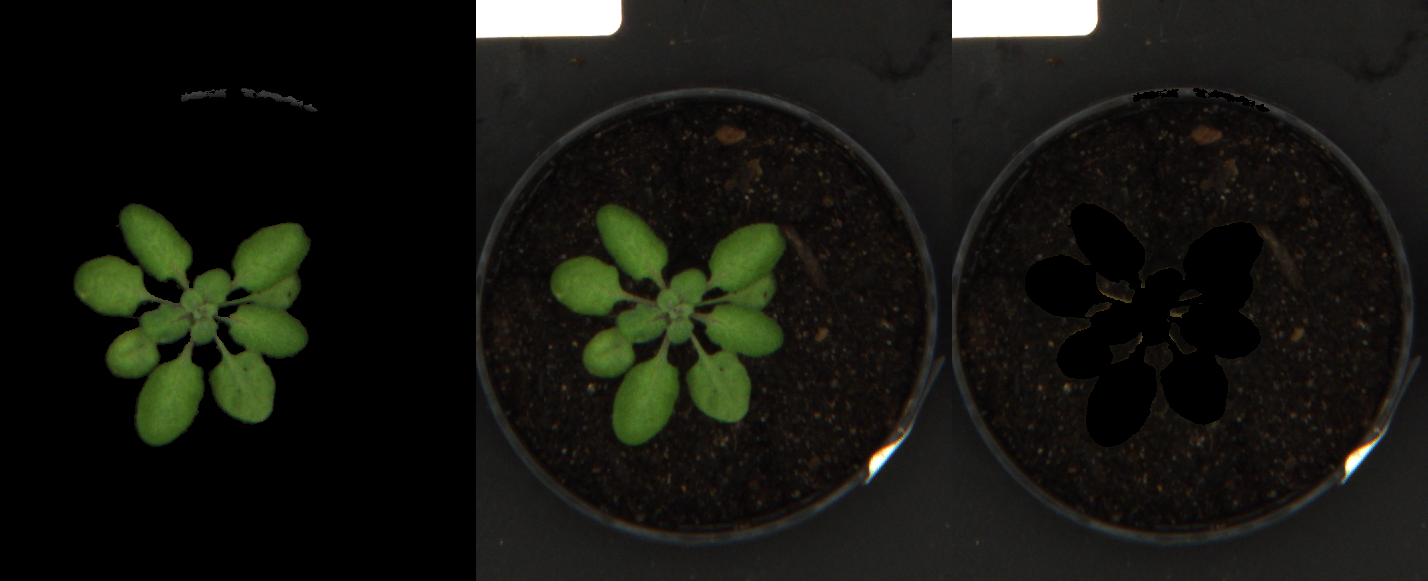
\includegraphics[width=10cm]{Figure1.png}
\end{center}
 \caption{Example of Arabidopsis thaliana Segmentation Left). Plant pixels. Center) Original Image. Right) Background pixels}\label{fig1:segmentation}
\end{figure}

\begin{figure}[h!]
\begin{center}
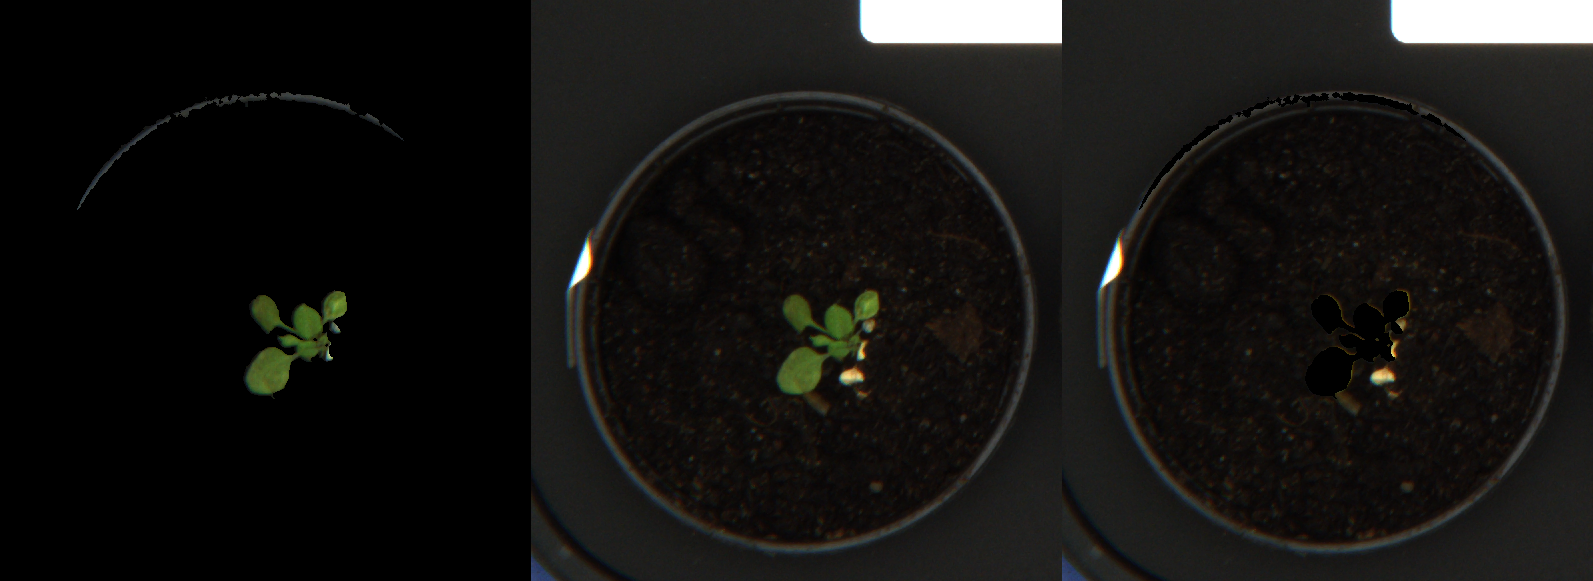
\includegraphics[width=10cm]{Figure2.png}
\end{center}
 \caption{Example of Arabidopsis Segmentation with segmentation errors Left) Foreground as plant pixels (True Positives) including pot border pixels as artefacts (False Positives). Centre) Original image. Left) Background pixels (True Negatives) including a yellow leaf and spots belonging to a turning yellow leaf (False Negatives).}\label{fig1:segmentation}
\end{figure}

%
%\begin{figure}[h!]
%\begin{center}
%\includegraphics[width=10cm]{flagleafsenescence.png}
%\end{center}
% \caption{Disease severity vs onset of senescence at the Flag Leaf. Red dots indicate average DAS per disease score}\label{fig2}
%\end{figure}
%
%
%\begin{figure}
%    \begin{center}
%    \begin{subfigure}[b]{0.5\textwidth}
%        \includegraphics[width=\textwidth]{W8-214112.png}
%        \caption{Early senescence, IT = 4}
%       % \label{fig:tiger}
%    \end{subfigure}
%    ~ %add desired spacing between images, e. g. ~, \quad, \qquad, \hfill etc. 
%    %(or a blank line to force the subfigure onto a new line)
%    \begin{subfigure}[b]{0.5\textwidth}
%        \includegraphics[width=\textwidth]{W8-100112.png}
%        \caption{Late senescence, IT = 4}
%        %\label{fig:mouse}
%    \end{subfigure}
%\end{center}
%    \caption{Contrast beween two lines whose disease score was four. Red vertical line indicates the date senescence on Flag leaf was first seen}\label{fig3}
%%\textbf{\refstepcounter{figure}\label{fig:03} Figure \arabic{figure}.}{Contrast beween two lines whose disease score was four. Red vertical line indicates the date senescence on Flag leaf was first seen}
%\end{figure}
%
%
%\begin{figure}
%    \begin{center}
%    \begin{subfigure}[b]{1\textwidth}
%        \includegraphics[width=\textwidth]{gs39_qtl.png}
%        \caption{}
%        \label{fig:gs39}
%    \end{subfigure}
%    ~ %add desired spacing between images, e. g. ~, \quad, \qquad, \hfill etc. 
%    %(or a blank line to force the subfigure onto a new line)
%\begin{subfigure}[b]{1\textwidth}
%        \includegraphics[width=\textwidth]{firstearweight_qtl.png}
%        \caption{}
%       \label{fig:firstearweight}
%    \end{subfigure}
%    ~ %add desired spacing between images, e. g. ~, \quad, \qquad, \hfill etc. 
%    %(or a blank line to force the subfigure onto a new line)
%    \begin{subfigure}[b]{1\textwidth}
%        \includegraphics[width=\textwidth]{thirdearlength_qtl.png}
%        \caption{}
%        \label{fig:thirdearlength}
%    \end{subfigure}
%\end{center}
%    \caption{QTLs hits for the taits gs39, first.ear.weightt and third.ear.length}\label{fig4}
%%\textbf{\refstepcounter{figure}\label{fig:03} Figure \arabic{figure}.}{Contrast beween two lines whose disease score was four. Red vertical line indicates the date senescence on Flag leaf was first seen}


%\end{figure}


%\begin{figure}
%\begin{center}
%\includegraphics[width=10cm]{logo2}% This is an *.eps file
%\end{center}
%\textbf{\refstepcounter{figure}\label{fig:02} Figure \arabic{figure}.}{ Enter the caption for your figure here.  Repeat as  necessary for each of your figures }
%\end{figure}

%%% If you don't add the figures in the LaTeX files, please upload them when submitting the article.

%%% Frontiers will add the figures at the end of the provisional pdf automatically %%%

%%% The use of LaTeX coding to draw Diagrams/Figures/Structures should be avoided. They should be external callouts including graphics.
\end{document}
